\documentclass[aspectratio=169, 11pt]{beamer}

% ========== 主题设置 ==========
\usetheme{Madrid}
\usecolortheme{whale}
\setbeamertemplate{navigation symbols}{}
\setbeamertemplate{footline}[frame number]

% ========== 包 ==========
\usepackage{tikz}
\usetikzlibrary{arrows.meta, positioning, shapes.geometric, calc, fit, backgrounds}
\usepackage{booktabs}
\usepackage{graphicx}
\usepackage{amsmath}
\usepackage{xcolor}

% ========== 颜色定义 ==========
\definecolor{highlight}{RGB}{255, 100, 100}      % 当前工作模块(红色高亮)
\definecolor{completed}{RGB}{100, 200, 100}      % 已完成模块(绿色)
\definecolor{pending}{RGB}{200, 200, 200}        % 待完成模块(灰色)
\definecolor{inprogress}{RGB}{100, 150, 255}     % 进行中(蓝色)

% ========== 标题信息 ==========
\title{Weekly Progress Report}
\subtitle{Week X: [本周主题]}
\author{Student ID: 11314389}
\institute{BCI Control System Project}
\date{\today}

\begin{document}

% ========== 标题页 ==========
\begin{frame}
    \titlepage
\end{frame}

% ========== Slide 1: 系统架构图 ==========
\begin{frame}{System Overview: Current Focus}
    \begin{center}
    \resizebox{0.95\textwidth}{!}{%
    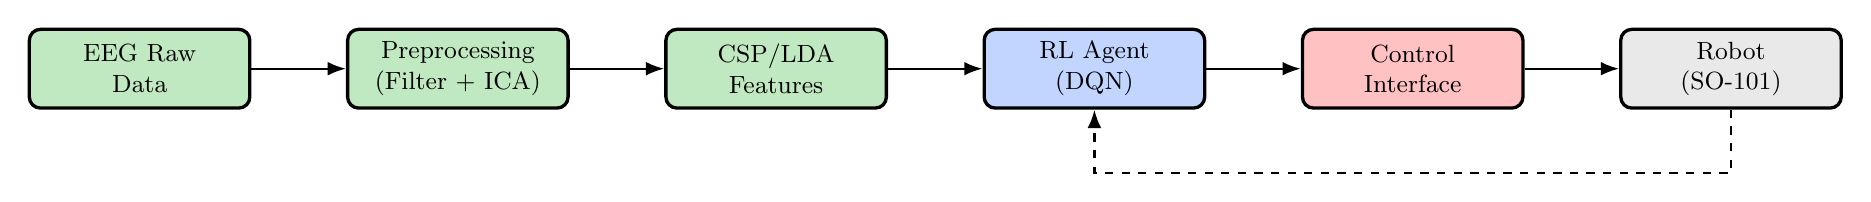
\begin{tikzpicture}[
        node distance=8mm and 12mm,
        block/.style={rectangle, rounded corners, draw, very thick,
                      minimum width=28mm, minimum height=10mm,
                      align=center, font=\small},
        arrow/.style={-Latex, thick},
    ]
        % ===== 修改这里来高亮当前工作的模块 =====
        % 状态: completed (绿), inprogress (蓝), highlight (红), pending (灰)
        
        \node[block, fill=completed!40] (raw) {EEG Raw\\Data};
        \node[block, fill=completed!40, right=of raw] (prep) {Preprocessing\\(Filter + ICA)};
        \node[block, fill=completed!40, right=of prep] (csp) {CSP/LDA\\Features};
        \node[block, fill=inprogress!40, right=of csp] (dqn) {RL Agent\\(DQN)};
        \node[block, fill=highlight!40, right=of dqn] (ctrl) {Control\\Interface};
        \node[block, fill=pending!40, right=of ctrl] (robot) {Robot\\(SO-101)};
        
        \draw[arrow] (raw) -- (prep);
        \draw[arrow] (prep) -- (csp);
        \draw[arrow] (csp) -- (dqn);
        \draw[arrow] (dqn) -- (ctrl);
        \draw[arrow] (ctrl) -- (robot);
        
        % 反馈回路
        \draw[arrow, dashed] (robot.south) -- ++(0,-8mm) -| (dqn.south);
        
    \end{tikzpicture}}
    \end{center}
    
    \vspace{3mm}
    \begin{columns}[T]
        \column{0.5\textwidth}
        \textbf{Legend:}
        \begin{itemize}
            \item[\textcolor{completed}{\rule{8pt}{8pt}}] Completed
            \item[\textcolor{inprogress}{\rule{8pt}{8pt}}] In Progress
        \end{itemize}
        \column{0.5\textwidth}
        \begin{itemize}
            \item[\textcolor{highlight}{\rule{8pt}{8pt}}] \textbf{This Week's Focus}
            \item[\textcolor{pending}{\rule{8pt}{8pt}}] Pending
        \end{itemize}
    \end{columns}
\end{frame}

% ========== Slide 2: 本周目标 ==========
\begin{frame}{This Week's Objectives}
    \begin{block}{Goals}
        \begin{enumerate}
            \item 目标 1: [例如:完成 RL 训练流程]
            \item 目标 2: [例如:测试 PyBullet 仿真环境]
            \item 目标 3: [例如:优化控制平滑度]
        \end{enumerate}
    \end{block}
    
    \vspace{5mm}
    
    \begin{alertblock}{Key Question to Address}
        [本周要回答的核心问题,例如:RL 策略能否产生比 CNN 更平滑的控制轨迹?]
    \end{alertblock}
\end{frame}

% ========== Slide 3: 方法/实现 ==========
\begin{frame}{Methods \& Implementation}
    \begin{columns}[T]
        \column{0.5\textwidth}
        \textbf{Approach:}
        \begin{itemize}
            \item 使用的技术/算法
            \item 关键参数设置
            \item 代码模块说明
        \end{itemize}
        
        \vspace{3mm}
        \textbf{Key Formula:}
        \begin{equation*}
            Q(s,a) \leftarrow r + \gamma \max_{a'} Q(s',a')
        \end{equation*}
        
        \column{0.5\textwidth}
        \textbf{Implementation Details:}
        \begin{itemize}
            \item \texttt{gym\_control.py}: 仿真环境
            \item \texttt{phy\_control.py}: 硬件控制
            \item 训练参数: $\gamma=0.99$, $\varepsilon$-decay
        \end{itemize}
    \end{columns}
\end{frame}

% ========== Slide 4: 结果 ==========
\begin{frame}{Results}
    \begin{columns}[T]
        \column{0.55\textwidth}
        \textbf{Quantitative Results:}
        
        \vspace{2mm}
        \begin{table}
            \centering
            \small
            \begin{tabular}{lcc}
                \toprule
                Metric & Baseline & This Week \\
                \midrule
                Accuracy & 72.3\% & 75.1\% \\
                Control Smoothness & 0.45 & 0.32 \\
                Success Rate & -- & 68\% \\
                \bottomrule
            \end{tabular}
        \end{table}
        
        \column{0.45\textwidth}
        \textbf{Visualization:}
        
        % 在这里插入图片
        % \includegraphics[width=\textwidth]{outputs/gym_summary.png}
        
        \begin{center}
            \fbox{\parbox{0.8\textwidth}{\centering\vspace{15mm}[Insert Figure Here]\vspace{15mm}}}
        \end{center}
    \end{columns}
    
    \vspace{3mm}
    \textbf{Key Observations:}
    \begin{itemize}
        \item 观察 1: [例如:RL 策略减少了 29\% 的方向抖动]
        \item 观察 2: [例如:在 Subject 3 上表现最好]
    \end{itemize}
\end{frame}

% ========== Slide 5: 挑战与解决 ==========
\begin{frame}{Challenges \& Solutions}
    \begin{columns}[T]
        \column{0.5\textwidth}
        \begin{alertblock}{Challenges Encountered}
            \begin{itemize}
                \item 问题 1: [例如:串口通信延迟]
                \item 问题 2: [例如:RL 收敛慢]
            \end{itemize}
        \end{alertblock}
        
        \column{0.5\textwidth}
        \begin{exampleblock}{Solutions Applied}
            \begin{itemize}
                \item 解决 1: [例如:增加缓冲区]
                \item 解决 2: [例如:调整学习率]
            \end{itemize}
        \end{exampleblock}
    \end{columns}
\end{frame}

% ========== Slide 6: 下周计划 ==========
\begin{frame}{Next Week's Plan}
    \begin{block}{Planned Tasks}
        \begin{enumerate}
            \item 任务 1: [例如:在真实机械臂上测试]
            \item 任务 2: [例如:收集跨被试泛化数据]
            \item 任务 3: [例如:撰写实验部分文档]
        \end{enumerate}
    \end{block}
    
    \vspace{5mm}
    
    \begin{columns}[T]
        \column{0.5\textwidth}
        \textbf{Expected Deliverables:}
        \begin{itemize}
            \item 物理机械臂演示视频
            \item 9 个被试的准确率表格
        \end{itemize}
        
        \column{0.5\textwidth}
        \textbf{Questions for Supervisor:}
        \begin{itemize}
            \item [需要讨论的问题]
            \item [需要的资源/帮助]
        \end{itemize}
    \end{columns}
\end{frame}

% ========== Slide 7: 时间线 ==========
\begin{frame}{Project Timeline}
    \begin{center}
    \resizebox{0.9\textwidth}{!}{%
    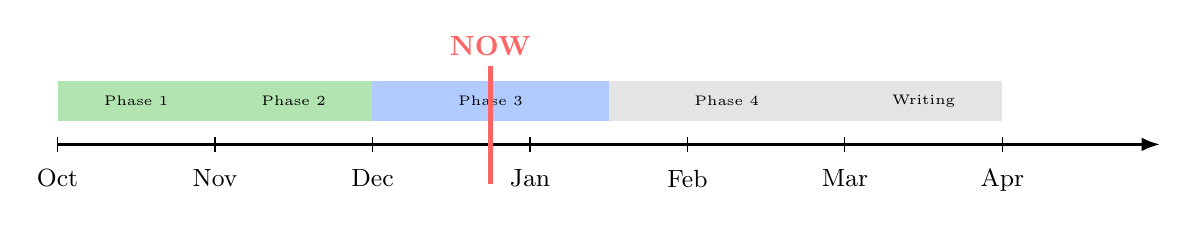
\begin{tikzpicture}
        % 时间轴
        \draw[thick, -Latex] (0,0) -- (14,0);
        
        % 月份标记
        \foreach \x/\month in {0/Oct, 2/Nov, 4/Dec, 6/Jan, 8/Feb, 10/Mar, 12/Apr} {
            \draw (\x, 0.1) -- (\x, -0.1);
            \node[below] at (\x, -0.2) {\small \month};
        }
        
        % 阶段块
        \fill[completed!50] (0, 0.3) rectangle (2, 0.8);
        \node at (1, 0.55) {\tiny Phase 1};
        
        \fill[completed!50] (2, 0.3) rectangle (4, 0.8);
        \node at (3, 0.55) {\tiny Phase 2};
        
        \fill[inprogress!50] (4, 0.3) rectangle (7, 0.8);
        \node at (5.5, 0.55) {\tiny Phase 3};
        
        \fill[pending!50] (7, 0.3) rectangle (10, 0.8);
        \node at (8.5, 0.55) {\tiny Phase 4};
        
        \fill[pending!50] (10, 0.3) rectangle (12, 0.8);
        \node at (11, 0.55) {\tiny Writing};
        
        % 当前位置
        \draw[highlight, ultra thick] (5.5, -0.5) -- (5.5, 1);
        \node[highlight, above] at (5.5, 1) {\textbf{NOW}};
        
    \end{tikzpicture}}
    \end{center}
    
    \vspace{3mm}
    \textbf{Current Status:} On track / Ahead / Behind schedule
\end{frame}

% ========== 备用: Demo Slide ==========
\begin{frame}{Demo / Video}
    \begin{center}
        % 插入演示截图或视频链接
        \fbox{\parbox{0.7\textwidth}{\centering\vspace{30mm}[Demo Screenshot / Video Link]\vspace{30mm}}}
        
        \vspace{5mm}
        \textit{Demo: [描述演示内容]}
    \end{center}
\end{frame}

\end{document}

